\documentclass{article}
\usepackage{graphicx} % Required for inserting images
\usepackage[a4paper, total={6in, 8in}, margin=1in]{geometry}
\usepackage{listings}
\usepackage{hyperref}
\usepackage{amsmath}
\usepackage{amssymb}
\usepackage{authblk}
\usepackage{float}
\usepackage{parskip}
\usepackage{minted}
\usepackage{fontawesome}
\usemintedstyle{vs}
\newcommand{\ts}{\textsuperscript}



\begin{document}

\begin{titlepage}
    \centering
    \vspace*{1cm}
    
    % Insert image (adjust width as needed)
    
    
    
    
    % Title
    {\Huge\bfseries INF219 – COWI Research \par}
    
    
    \vspace{1.5cm}
    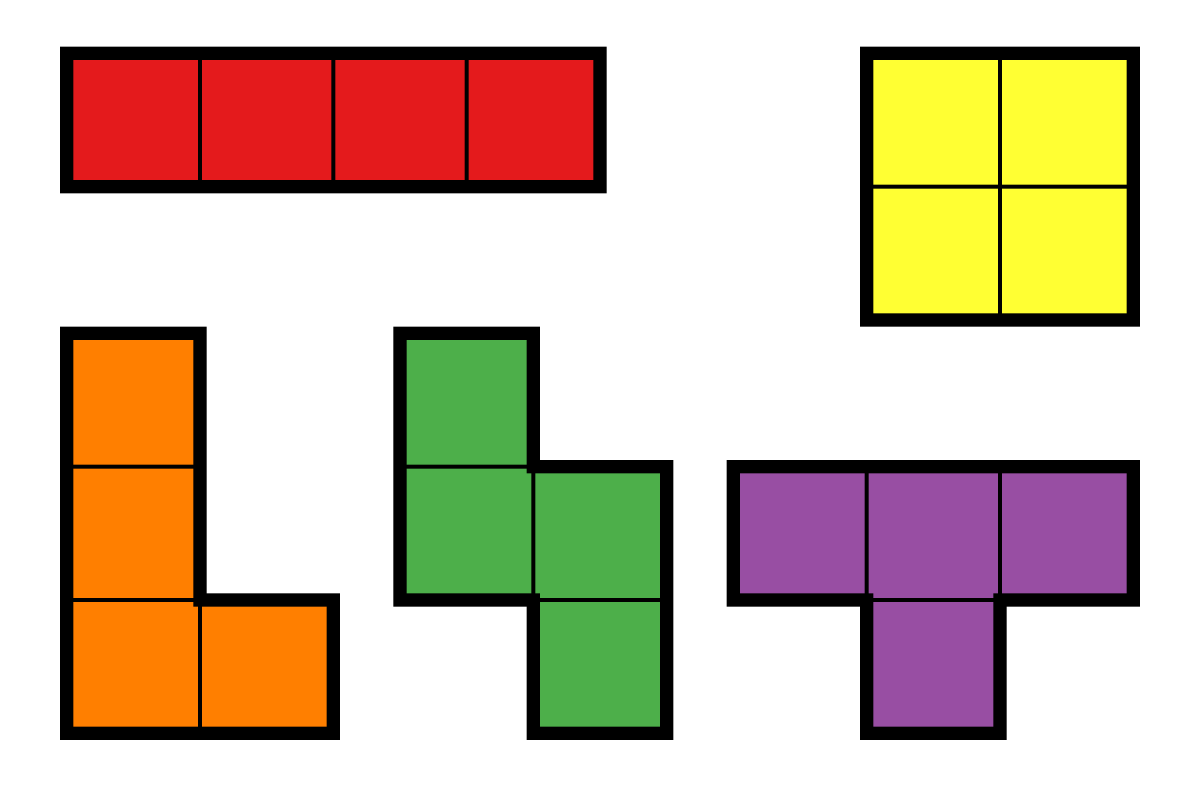
\includegraphics[width=0.5\textwidth]{tetris.png} % replace with your image file name
    \vspace{1cm}
    % Authors

    {\large Jakob Sverre Alexandersen \\
    Thone Anlaug Stordal Støa \\
    Hanna Søndenaa Rasmussen \\
    Håvard Kattem Lunde \\
    Hermann Holstad Walaunet \par}
    
    
    \vfill
    
    % Footer
    {\large April 2025 \par}
    
    \vspace{1cm}
    \href{https://github.com/alexandersen01/COWI-research}{\faicon{github} GitHub Repository}
\end{titlepage}


\newpage

\tableofcontents

\newpage

\section{Summary}

Click me: \href{https://github.com/alexandersen01/COWI-research}{\faicon{github}} for the full repo

\hrulefill{}

This project considers techniques for placing light fixtures in any given room, 
minimizing the amount of lights used whilst still being compliant with regulatory
and aesthetic requirements.

There are many different approaches to such a challenge. For instance, COWI presented
a genetic algorithm/reinforcement learning ML-based solution. Their apprach 
entailed maximizing coverage area while maintaining a pattern by penalizing variations
in x/y coordinates. 

We chose to take a different approach, using Linear Programming instead. The main reason
behind this choice is the guaranteed optimality involved in such a solution.
Using a solver, we are able to find the single most mathematically optimal solution 
that satisfies all constraints, given that a solution exists.

In addition to the optimality, we are also presented with several other advantages 
using the LP approach. The deterministic nature of our solution ensures that given 
the same inputs and constraints, we always get identical, reproducible 
results — eliminating the randomness inherent in genetic algorithms. This 
consistency is particularly valuable in professional settings where repeatability 
is essential.

Our LP formulation also offers greater transparency and explainability, making it 
clear exactly what we're optimizing for and what constraints we're satisfying. 
For typical room dimensions, the LP solver finds optimal solutions relatively quickly, 
without requiring the multiple generations of evolution that genetic algorithms need. 
This efficiency translates to faster design iterations and project delivery.
The precise constraint handling in our approach allows for explicit modeling of 
critical requirements like minimum light levels and fixture spacing. Rather than 
approximating these through penalty functions as in the genetic algorithm approach, 
we incorporate them directly into the mathematical model.
Finally, our solution offers straightforward adaptability to changing requirements. 
The LP model parameters can be easily adjusted to meet different regulatory 
standards or design preferences without needing to retrain an entire ML model. 
While the ML-based approach might offer advantages in terms of continuous 
learning from historical data, our LP solution provides immediate, verifiable 
results with mathematical guarantees—a critical factor when dealing with 
safety-related regulatory compliance in building design. This becomes a bigger deal
if we choose to also incorporate positioning of a sprinkler system.

\newpage

\section{Motivation and Introduction (Thone)}

\newpage

\section{Mathematics (jakob se over)}

In this section, we will discuss the mathematical model behind the program.

\subsection{Sets and Indices}

\begin{align}
    G = (x, y) \mid (x, y) \in \mathbb{R}
\end{align}
\begin{align}
    A = (x, y) \mid (x, y) \in \mathbb{R}
\end{align}

\subsection{Decision Variables}

\begin{align}
    z_{x, y} \in \{0, 1\} \text{ for } (x, y) \in G
\end{align}
\begin{align}
    c_{x, y} \geq 0 \text{ for } (x, y) \in G
\end{align}

\subsection{Parameters}

\begin{align}
    \alpha_{(x_g, y_g), (x_a, y_a)} \in \{0, 1\}
\end{align}
\begin{align}
    L_{\min} \geq 0
\end{align}
\begin{align}
        S_{\min} \geq 0
\end{align}
\begin{align}
    A_g
\end{align}

\subsection{Objective Function}

\begin{align}
    \min \sum_{(x, y) \in G} z_{x, y}
\end{align}

\subsection{Constraints}

\begin{align}
    c_{x_a, y_a} = \sum_{(x, y) \in G} \alpha_{(x_g, y_g), {x_a, y_a}} \cdot z_{x_g, y_g} \quad\forall (x_a, y_a) \in A
\end{align}
\begin{align}
    \sum_{(x_a, y_a) \in A_g} c_{x_a, y_a} \geq L_{\min} \cdot |A_g| \quad\forall g \in G \text{ where } |A_g| > 0
\end{align}
\begin{align}
    \max \bigg(\frac{|x_1 - x_2|}{\text{grid size}}, \frac{|y_1 - y_2|}{\text{grid size}}\bigg) \leq S_{\min}
\end{align}
\begin{align}
    z_{x_1, y_1} + z_{x_2, y_2} \leq 1
\end{align}

\newpage

\subsection{Equations explainations}

\begin{enumerate}
    \item List of grid points where we may place light fixtures
    \item List of smaller grid points used to calculate the coverage
    \item Binary variable indicating whether a light is placed at point $(x, y)$ – $1$ if yes, $0$ otherwise
    \item Continuous variable representing the light level at area cell $(x, y)$
    \item Coverage value representing the amount of light that a fixture at grid point $(x_g,y_g)$ contributes to area cell $(x_a,y_a)$
    \item Minimum average light level required in each grid cell
    \item Minimum spacing required between fixtures (measured in grid units)
    \item Set of area cells contained within the grid cell $g \in G$
    \item \textbf{Minimize the total amount of light fixtures}
    \item For each area cell $(x_a,y_a) \in A$, the light level is determined by the sum of contributions from all placed fixtures
    \item For each grid cell $(x_g,y_g) \in G$, the average light level across all contained area cells must meet or exceed the minimum requirement
    \item For any two grid points $(x_1,y_1), (x_2,y_2) \in G$ that are closer than the minimum spacing,
    \item We add the constraint that at most one of them can have a fixture
    \item TODO: add neigh constraint 
\end{enumerate}

\newpage

\section{Execution}
\subsection{Method (jakob)}
\subsection{What we tried: (hanna)}

\newpage

\section{Experiments (TBD)}
\subsection{Light distribution plot}
\subsection{Small room}
\subsection{Large room}
\subsection{Runtime Discussion}



\newpage

\section{Discussion (Håvard)}

\subsection{Potential Improvements}
\subsubsection{Caching}

\newpage

\section{Conclusion (Hermann)}

In this project, we have explored two approaches to lighting optimization using the PuLP library, a mixed-integer programming solver.
The first model uses a simple mathematical grid patterning approach that places lights based on fixed spacing rules, independent of actual lighting values.
This results in visually good, regular arrangements, but lacks adaptability to lighting requirements.

The second model is a constraint-based optimization solution that mathematically ensures compliance with lighting thresholds,
fixture spacing, and other constraints. This model provides precise results and guarantees that the lighting meets the minimum lux requirement
throughout the room. However, the output can sometimes appear less pleasing, especially in irregular spaces, as the focus is purely on optimization rather than visual symmetry.

Through our experiments, we observed that the optimization model performs particularly well when the required lighting level is higher,
such as 300 lux or more. In such cases, the denser fixture placement leaves more room for the solver to balance aesthetics and coverage.
Conversely, at low lux requirements, the model tends to use fewer lights and may produce more irregular patterns.

The project was carried out through structured collaboration, with group meetings and division of tasks ensuring even distribution of work 
and collective problem-solving. Together, we have demonstrated how linear programming can be a powerful tool
in practical engineering contexts, offering both adaptability and mathematical rigor.


\end{document}